%!TEX TS-program = xelatex
%!TEX encoding = UTF-8 Unicode

\documentclass[a4paper,11pt]{article}


\usepackage{fontspec}

\setmainfont{Linux Libertine}
% \setmainfont{Arial}
% \setmainfont{DejaVu Sans}
% \setmainfont{Georgia}
% \setmainfont{Times New Roman}

\setmonofont{Consolas}[Scale=MatchLowercase]
% \setmonofont{Droid Sans Mono}[Scale=MatchLowercase]
% \setmonofont{Courier New}[Scale=MatchLowercase]

 
\usepackage{listings}
\lstset{%
	language=Java,
	basicstyle=\footnotesize\ttfamily,
	frame=single,
	breaklines=true,
	showstringspaces=false
}


\usepackage{graphicx}
\graphicspath{ {images/} }

\usepackage{hyperref}

\title{Android Client}
\author{Καμπυλαυκάς Ιωάννης \\ sdi9500781@di.uoa.gr \and Σούλης Αθανάσιος \\ sdi0900155@di.uoa.gr}
\date{2 Φεβρουαρίου 2015}
\renewcommand{\contentsname}{Περιεχόμενα}
\renewcommand{\figurename}{Σχήμα}

\begin{document}

\begin{sloppypar}

\maketitle

\tableofcontents

\newpage


\section{Οι προσθήκες στον Aggregator Manager}



\begin{figure}[h]
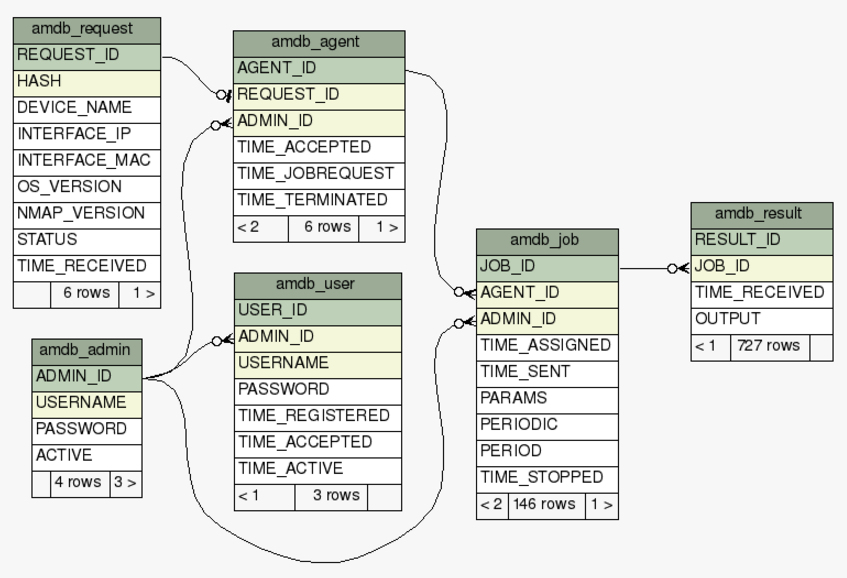
\includegraphics[width=\textwidth]{schema}
\centering
\caption{Το ενημερωμένο σχήμα της βάσης δεδομένων του Aggregator Manager.}
\end{figure}


\subsection{Σχήμα της βάσης δεδομένων}

Στους υπάρχοντες πίνακες από το δεύτερο μέρος του project προστέθηκε ο πίνακας των χρηστών των Android Clients, amdb\_users. Τα πεδία του είναι τα εξής:

\begin{itemize}

\item USER\_ID: πρωτεύον κλειδί του πίνακα, δημιουργείται αυτόματα.

\item ADMIN\_ID: ξένο κλειδί στον πίνακα των διαχειριστών του Aggregator Manager. Όταν είναι NULL, ο χρήστης δεν έχει εγκριθεί από κάποιον διαχειριστή. Όταν κάποιος διαχειριστής εγκρίνει έναν χρήστη, τότε το πεδίο παίρνει την τιμή του αναγνωριστικού του διαχειριστή.

\item USERNAME: το όνομα του χρήστη. Υπάρχει περιορισμός μοναδικότητας της τιμής του πεδίου αυτού για τον πίνακα, όπως και στο αντίστοιχο πεδίο του πίνακα των διαχειριστών.

\item PASSWORD: το συνθηματικό του χρήστη. Δεν αποθηκεύεται αυτούσιο το συνθηματικό αλλά η έξοδος του αλγορίθμου SHA256 με είσοδο το συνθηματικό. 

\item TIME\_REGISTERED: είναι η χρονική στιγμή της εγγραφής του χρήστη στη βάση δεδομένων.

\item TIME\_ACCEPTED: είναι η χρονική στιγμή της αποδοχής του χρήστη από κάποιον διαχειριστή. Στην περίπτωση που ο χρήστης δεν έχει γίνει ακόμη αποδεκτός έχει την τιμή NULL. Την τιμή NULL παίρνει και αν κάποιος διαχειριστής απορρίψει εκ των υστέρων έναν χρήστη που έχει γίνει αρχικά αποδεκτός.

\item TIME\_ACΤIVE: είναι η χρονική στιγμή της τελευταίας χρήσης των υπηρεσιών του Aggregator Manager από τον χρήστη.

\end{itemize}
Όταν ένας χρήστης αναθέσει μια εργασία σε κάποιον Software Agent, αυτή δημιουργείται εκ μέρους του διαχειριστή που έχει εγκρίνει τον χρήστη. Η δημιουργία εργασιών γίνεται τελικά μόνο από διαχειριστές του Aggregator Manager, όπως και στο δεύτερο μέρος του project. 
\\
Στη γραφική διεπαφή για τον Aggregator Manager έχει προστεθεί η αναγκαία όψη για την αποδοχή ή απόρριψη χρηστών από κάποιον διαχειριστή.

\subsection{Ρυθμίσεις}

Στις ρυθμίσεις του Aggregator Manager έχουν προστεθεί οι εξής, σχετικές με τη δραστηριότητα των απομακρυσμένων χρηστών.
\\

\noindent\begin{tabular}{lp{11cm}}

\texttt{expireUserSessions=true}\\
\texttt{userSessionMinutes=30}\\
\end{tabular}
\\

Η ρύθμιση userSessionMinutes καθορίζει για πόσα λεπτά μπορεί να μείνει ενεργός ένας χρήστης Android Client χωρίς να χρησιμοποιήσει κάποια από τις υπηρεσίες του Aggregator Manager. Μετά την παρέλευση του χρόνου αυτού ο Aggregator Manager δεν επιστρέφει δεδομένα στα αιτήματα του χρήστη. Η ρύθμιση αυτή λαμβάνεται υπ' όψιν μόνο στην περίπτωση που η ρύθμιση expireUserSessions είναι ενεργή. Σε αντίθετη περίπτωση, ο Aggregator Manager επιστρέφει πάντοτε δεδομένα σε κάθε αίτημα ενός Android Client με έγκυρες παραμέτρους και η ρύθμιση userSessionMinutes χρησιμοποιείται μόνο στην όψη των χρηστών της γραφικής διεπαφής του Aggregator Manager, για να τους χαρακτηρίσει ενεργούς ή ανενεργούς.

\newpage

\subsection{Οι REST υπηρεσίες για τους Android Clients}

Στον Aggregator Manager έχει προστεθεί η κλάση ClientHandlers που αφορά στην επικοινωνία των Android Clients με αυτόν. Οι υπηρεσίες που περιλαμβάνει είναι οι εξής:

\subsubsection{Εγγραφή}
\begin{lstlisting}
@GET
@Path("register/{username}/{password}")
@Produces(MediaType.TEXT_PLAIN)
public Response register(
    @PathParam("username") String username,
    @PathParam("password") String password) {
    ...
}
\end{lstlisting}
Η μέθοδος register() ακούει σε ένα URI της μορφής:
\\
\url{http://localhost:8080/am/client/register/{username}/{password}}
\\
για ένα αίτημα εγγραφής νέου χρήστη Android Client.
\begin{itemize}

\item username: το όνομα του νέου χρήστη.
\item password: το συνθηματικό του χρήστη.
\end{itemize}
Οι πιθανές απαντήσεις του AM είναι:
\begin{itemize}
\item "Registration Success", στην περίπτωση επιτυχούς εγγραφής.
\item "User Exists", αν υπάρχει ήδη χρήστης με το όνομα που δόθηκε.
\item "Service Error", στην περίπτωση οποιουδήποτε άλλου σφάλματος.
\end{itemize}
Αν το όνομα του νέου χρήστη δεν υπερβαίνει το μέγιστο μέγεθος και δεν υπάρχει ήδη χρήστης με αυτό το όνομα, τότε η εγγραφή είναι επιτυχής. Ο χρήστης πρέπει να εγκριθεί από κάποιον διαχειριστή προτού να μπορέσει να συνδεθεί επιτυχώς μέσω της υπηρεσίας σύνδεσης.

\subsubsection{Σύνδεση}
\begin{lstlisting}
@GET
@Path("login/{username}/{password}")
@Produces(MediaType.TEXT_PLAIN)
public Response login(
    @PathParam("username") String username,
    @PathParam("password") String password) {
    ...
}

\end{lstlisting}
Η μέθοδος login() ακούει σε ένα URI της μορφής:
\\
\url{http://localhost:8080/am/client/login/{username}/{password}}
\\
για ένα αίτημα σύνδεσης χρήστη Android Client.

\begin{itemize}

\item username: το όνομα του χρήστη.
\item password: το συνθηματικό του χρήστη.

\end{itemize}
Οι πιθανές απαντήσεις του AM είναι:
\begin{itemize}
\item "Login Success", στην περίπτωση επιτυχούς σύνδεσης.
\item "Incorrect Credentials", αν τα στοιχεία χρήστη είναι μη έγκυρα.
\item "Registration Pending", αν ο χρήστης δεν έχει εγκριθεί ακόμη.
\item "Service Error", στην περίπτωση οποιουδήποτε άλλου σφάλματος.
\end{itemize}
Αν τα στοιχεία είναι έγκυρα, ενημερώνεται το πεδίο TIME\_ACTIVE της εγγραφής που αντιστοιχεί στον χρήστη και στο εξής ο χρήστης μπορεί να στέλνει αιτήματα στις υπόλοιπες υπηρεσίες του Aggregator Manager με μέγιστο χρονικό διάστημα μεταξύ αιτημάτων όσο καθορίζεται από την ρύθμιση userSessionMinutes του AM. Αν αυτό το χρονικό διάστημα ξεπεραστεί, απαιτείται νέα σύνδεση του χρήστη.

\subsubsection{Λήψη Software Agents}
\begin{lstlisting}
@GET
@Path("agents/{username}/{password}")
@Produces(MediaType.APPLICATION_XML)
public Response agents(
    @PathParam("username") String username,
    @PathParam("password") String password) {
    ...
}
\end{lstlisting}
Η μέθοδος agents() ακούει σε ένα URI της μορφής:
\\
\url{http://localhost:8080/am/client/agents/{username}/{password}}
\\
για ένα αίτημα χρήστη για τους Software Agents που υπάρχουν στη βάση του Aggregator Manager.
\begin{itemize}

\item username: το όνομα του νέου χρήστη.
\item password: το συνθηματικό του χρήστη.

\end{itemize}
Ένα παράδειγμα απάντησης της υπηρεσίας είναι το εξής:
\newpage


\begin{lstlisting}
<?xml version="1.0" encoding="UTF-8" standalone="yes"?>
<agents status="Accepted" >
  <agent>
    <agentId>4</agentId>
    <requestHash>
      C886C27EF2CA686311C6918FA43B0AF90D2F7FFBD73C2958D48D399D4E037563
    </requestHash>
    <timeAccepted>2016-01-28 22:36:21.0 EET</timeAccepted>
    <agentStatus>OFFLINE</agentStatus>
  </agent>
  <agent>
    <agentId>3</agentId>
    <requestHash>
      5A885FD0CEB82033480975B0203B632EE07E8E8B8B4421894969C2777D10D5D5
    </requestHash>
    <timeAccepted>2016-01-26 18:25:18.0 EET</timeAccepted>
    <timeJobRequest>2016-02-03 02:37:04.0 EET</timeJobRequest>
    <timeTerminated>2016-02-02 01:36:48.0 EET</timeTerminated>
    <agentStatus>ONLINE</agentStatus>
  </agent>
</agents>
\end{lstlisting}
Οι πιθανές τιμές του attribute status είναι οι εξής:
\begin{itemize}
\item "Accepted", αν το αίτημα έγινε δεκτό. Αυτή είναι η μόνη περίπτωση που επιστρέφονται δεδομένα (agents) στον Android Client.
\item "Session Expired", στην περίπτωση που ο χρόνος σύνδεσης έχει παρέλθει.
\item "Incorrect Credentials", αν τα στοιχεία χρήστη είναι μη έγκυρα.
\item "Registration Pending", αν ο χρήστης δεν έχει εγκριθεί ακόμη.
\item "Service Error", στην περίπτωση οποιουδήποτε άλλου σφάλματος.
\end{itemize}

\subsubsection{Λήψη των nmap jobs ενός Software Agent}
\begin{lstlisting}
@GET
@Path("jobs/{username}/{password}/{agentHash}")
@Produces(MediaType.APPLICATION_XML)
public Response jobs(
    @PathParam("username") String username,
    @PathParam("password") String password,
    @PathParam("agentHash") String agentHash) {
    ...
}
\end{lstlisting}
Η μέθοδος jobs() ακούει σε ένα URI της μορφής: \url{http://localhost:8080/am/client/jobs/{username}/{password}/{agentHash}} για ένα αίτημα χρήστη για τα jobs που έχουν ανατεθεί σε κάποιον Software Agent. Οι παράμετροι είναι:

\newpage

\begin{itemize}

\item username: το όνομα του χρήστη.
\item password: το συνθηματικό του χρήστη.
\item agentHash: το αναγνωριστικό του Software Agent.

\end{itemize}
Ένα παράδειγμα απάντησης της υπηρεσίας είναι το εξής:
\begin{lstlisting}
<?xml version="1.0" encoding="UTF-8" standalone="yes"?>
<jobs status="Accepted">
  <job>
    <jobId>11</jobId>
    <agentId>1</agentId>
    <adminId>4</adminId>
    <timeAssigned>2016-01-25 12:36:47.0 EET</timeAssigned>
    <params>-O -oX - 127.0.0.1</params>
    <periodic>true</periodic>
    <period>30</period>
  </job>
  <job>
    <jobId>27</jobId>
    <agentId>1</agentId>
    <adminId>4</adminId>
    <timeAssigned>2016-01-26 16:50:10.0 EET</timeAssigned>
    <params>-A -oX - 192.168.1.0/24</params>
    <periodic>false</periodic>
    <period>0</period>
  </job>
  <job>
    <jobId>28</jobId>
    <agentId>1</agentId>
    <adminId>4</adminId>
    <timeAssigned>2016-01-26 16:59:51.0 EET</timeAssigned>
    <params>stop 11</params>
    <periodic>false</periodic>
    <period>0</period>
  </job>
</jobs>
\end{lstlisting}
Οι πιθανές τιμές του attribute status είναι οι εξής:
\begin{itemize}
\item "Accepted", αν το αίτημα έγινε δεκτό. Αυτή είναι η μόνη περίπτωση που επιστρέφονται δεδομένα (jobs) στον Android Client.
\item "Invalid Hash", αν το αναγνωριστικό του Software Agent είναι μη έγκυρο.
\item "Session Expired", στην περίπτωση που ο χρόνος σύνδεσης έχει παρέλθει.
\item "Incorrect Credentials", αν τα στοιχεία χρήστη είναι μη έγκυρα.
\item "Registration Pending", αν ο χρήστης δεν έχει εγκριθεί ακόμη.
\item "Service Error", στην περίπτωση οποιουδήποτε άλλου σφάλματος.
\end{itemize}

\subsubsection{Λήψη τελευταίων αποτελεσμάτων ενός Software Agent}
\begin{lstlisting}
@GET
@Path("results/agent/{username}/{password}/{agentHash}/{number}")
@Produces(MediaType.APPLICATION_XML)
public Response agentResults(
    @PathParam("username") String username,
    @PathParam("password") String password,
    @PathParam("agentHash") String agentHash,
    @PathParam("number") int number) {
    ...
}
\end{lstlisting}
Η μέθοδος agentResults() ακούει σε ένα URI της μορφής:
\\
\url{http://localhost:8080/am/client/results/agent/{username}/{password}/{agentHash}/{number}} για ένα αίτημα χρήστη για τα τελευταία αποτελέσματα κάποιου Software Agent. Οι παράμετροι του αιτήματος είναι:
\begin{itemize}

\item username: το όνομα του χρήστη.
\item password: το συνθηματικό του χρήστη.
\item agentHash: το αναγνωριστικό του Software Agent.
\item number: το μέγιστο πλήθος των τελευταίων αποτελεσμάτων.
\end{itemize}
Ένα παράδειγμα απάντησης της υπηρεσίας είναι το εξής:
\begin{lstlisting}
<?xml version="1.0" encoding="UTF-8" standalone="yes"?>
<results status="Accepted">
  <result>
    <resultId>602</resultId>
    <jobId>9</jobId>
    <timeReceived>2016-01-24 14:14:11.0 EET</timeReceived>
    <output>
      &lt;?xml version="1.0"?&gt;
      &lt;nmaprun scanner="nmap" args="nmap -O -oX - 127.0.0.1"
      start="1453637628" startstr="Sun Jan 24 14:13:48 2016" version="6.47"
      ...
    </output>
  </result>
  <result>
    <resultId>603</resultId>
    <jobId>9</jobId>
    <timeReceived>2016-01-24 14:14:41.0 EET</timeReceived>
    <output>
      &lt;?xml version="1.0"?&gt;
      &lt;nmaprun scanner="nmap" args="nmap -O -oX - 127.0.0.1"
      start="1453637658" startstr="Sun Jan 24 14:14:18 2016" version="6.47"
      ...
    </output>
  </result>

  <result>
    <resultId>606</resultId>
    <jobId>9</jobId>
    <timeReceived>2016-01-24 14:16:11.0 EET</timeReceived>
    <output>
      &lt;?xml version="1.0"?&gt;
      &lt;nmaprun scanner="nmap" args="nmap -O -oX - 127.0.0.1"
      start="1453637748" startstr="Sun Jan 24 14:15:48 2016" version="6.47"
      ...
      &lt;/nmaprun&gt;
    </output>
  </result>
</results>
\end{lstlisting}
Οι πιθανές τιμές του attribute status είναι οι εξής:
\begin{itemize}
\item "Accepted", αν το αίτημα έγινε δεκτό. Αυτή είναι η μόνη περίπτωση που επιστρέφονται δεδομένα (results) στον Android Client.
\item "Invalid Hash", αν το αναγνωριστικό του Software Agent είναι μη έγκυρο.
\item "Session Expired", στην περίπτωση που ο χρόνος σύνδεσης έχει παρέλθει.
\item "Incorrect Credentials", αν τα στοιχεία χρήστη είναι μη έγκυρα.
\item "Registration Pending", αν ο χρήστης δεν έχει εγκριθεί ακόμη.
\item "Service Error", στην περίπτωση οποιουδήποτε άλλου σφάλματος.
\end{itemize}


\subsubsection{Λήψη τελευταίων αποτελεσμάτων για όλους τους Software Agents}
\begin{lstlisting}
@GET
@Path("results/all/{username}/{password}/{number}")
@Produces(MediaType.APPLICATION_XML)
public Response allResults(
    @PathParam("username") String username,
    @PathParam("password") String password,
    @PathParam("number") int number) {
    ...
}
\end{lstlisting}
Η μέθοδος allResults() ακούει σε ένα URI της μορφής:
\\
\url{http://localhost:8080/am/client/results/all/{username}/{password}/{number}} για ένα αίτημα χρήστη για τα τελευταία αποτελέσματα όλων των Software Agents. Οι παράμετροι του αιτήματος είναι:
\begin{itemize}

\item username: το όνομα του χρήστη.
\item password: το συνθηματικό του χρήστη.
\item number: το μέγιστο πλήθος των τελευταίων αποτελεσμάτων.
\end{itemize}
Ένα παράδειγμα απάντησης της υπηρεσίας είναι το εξής:
\begin{lstlisting}
<results status="Accepted">
  <result>
    <resultId>1370</resultId>
    <agentHash>
      5A885FD0CEB82033480975B0203B632EE07E8E8B8B4421894969C2777D10D5D5
    </agentHash>
    <jobId>119</jobId>
    <timeReceived>2016-01-29 23:16:34.0 EET</timeReceived>
    <output>
      &lt;?xml version="1.0"?&gt;
      &lt;nmaprun scanner="nmap" args="nmap -O -oX - 127.0.0.1"
      start="1454102163" startstr="Fri Jan 29 23:16:03 2016" version="6.47"
      xmloutputversion="1.04"&gt;
      ...
    </output>
  </result>
  <result>
    <resultId>1371</resultId>
    <agentHash>
      5A885FD0CEB82033480975B0203B632EE07E8E8B8B4421894969C2777D10D5D5
    </agentHash>
    <jobId>118</jobId>
    <timeReceived>2016-01-29 23:16:46.0 EET</timeReceived>
    <output>
      &lt;?xml version="1.0"?&gt;
      &lt;nmaprun scanner="nmap" args="nmap -O -oX - 127.0.0.1"
      start="1454102183" startstr="Fri Jan 29 23:16:23 2016" version="6.47"
      xmloutputversion="1.04"&gt;
      ...
    </output>
  </result>
  <result>
    <resultId>1372</resultId>
    <agentHash>
      85D4017BA2AD69140157A7E3E5F1A9576E9049B9ADD87AF51F278BE002780F62
    </agentHash>
    <jobId>116</jobId>
    <timeReceived>2016-01-29 23:20:09.0 EET</timeReceived>
    <output>
      &lt;?xml version="1.0"?&gt;
      &lt;nmaprun scanner="nmap" args="nmap -O -oX - 127.0.0.1"
      start="1453636968" startstr="Sun Jan 24 14:02:48 2016" version="6.47"
      xmloutputversion="1.04"&gt;
      ...
    </output>
  </result>
</results>
\end{lstlisting}

Οι πιθανές τιμές του attribute status είναι οι εξής:
\begin{itemize}
\item "Accepted", αν το αίτημα έγινε δεκτό. Αυτή είναι η μόνη περίπτωση που επιστρέφονται δεδομένα (jobs) στον Android Client.
\item "Session Expired", στην περίπτωση που ο χρόνος σύνδεσης έχει παρέλθει.
\item "Incorrect Credentials", αν τα στοιχεία χρήστη είναι μη έγκυρα.
\item "Registration Pending", αν ο χρήστης δεν έχει εγκριθεί ακόμη.
\item "Service Error", στην περίπτωση οποιουδήποτε άλλου σφάλματος.
\end{itemize}

\subsubsection{Ανάθεση εργασιών από απομακρυσμένους χρήστες}
\begin{lstlisting}
@POST
@Path("users/")
@Consumes(MediaType.APPLICATION_XML)
@Produces(MediaType.TEXT_PLAIN)
    public Response users(UserContainer userContainer) {
    ...
}
\end{lstlisting}
Η μέθοδος users() ακούει στο URI: \url{http://localhost:8080/am/client/users} για ένα αίτημα χρήστη με περιεχόμενο εργασίες προς ανάθεση σε Software Agents. Είναι η μόνη υπηρεσία που χρησιμοποιεί την HTTP μέθοδο POST με XML περιεχόμενο.
Ένα παράδειγμα περιεχομένου προς κατανάλωση από την υπηρεσία είναι το εξής:
\begin{lstlisting}
<users>
  <user username="Yannis"
password="0BFE935E70C321C7CA3AFC75CE0D0CA2F98B5422E008BB31C00C6D7F1F1C0AD6">
    <job>
      <agentId>3</agentId>
      <timeAssigned>2016-02-03 06:14:58.0 EET</timeAssigned>
      <params>stop 143</params>
      <periodic>false</periodic>
      <period>0</period>
    </job>
    <job>
      <agentId>3</agentId>
      <timeAssigned>2016-02-03 06:15:00.0 EET</timeAssigned>
      <params>-O -oX - 127.0.0.1</params>
      <periodic>true</periodic>
      <period>30</period>
    </job>
  </user>
  <user username="Thanos"
password="5994471ABB01112AFCC18159F6CC74B4F511B99806DA59B3CAF5A9C173CACFC5">
    <job>
      <agentId>4</agentId>
      <timeAssigned>2016-02-03 06:18:10.776 EET</timeAssigned>
      <params>exit</params>
      <periodic>false</periodic>
      <period>0</period>
    </job>
  </user>
</users>
\end{lstlisting}

Όπως φαίνεται στο παράδειγμα, το περιεχόμενο που αποστέλλεται στην υπηρεσία είναι ένα σύνολο χρηστών. Κάθε χρήστης συνοδεύεται από το όνομα και το συνθηματικό του και περιέχει ένα σύνολο εργασιών που επιθυμεί να αναθέσει σε κάποιον Software Agent. Οι πιθανές απαντήσεις της υπηρεσίας είναι:
\begin{itemize}
\item "Accepted", στην περίπτωση που η υπηρεσία επεξεργαστεί το περιεχόμενο επιτυχώς.
\item "Service Error", στην περίπτωση που συμβεί κάποιο σφάλμα κατά την επεξεργασία.
\end{itemize}

\newpage

\section{Ο Android Client}

\subsection{Εγγραφή - Σύνδεση}

Κατά την εκκίνησή του, ο Android Client ζητά τα στοιχεία σύνδεσης του χρήστη. Στην περίπτωση επιτυχούς σύνδεσης με την αντίστοιχη υπηρεσία του Aggregator Manager, τα στοιχεία σύνδεσης αποθηκεύονται σε shared preferences έτσι ώστε να είναι διαθέσιμα σε πιθανή μεταγενέστερη εκτέλεση του προγράμματος χωρίς να τα εισάγει ξανά ο χρήστης. Αν ο χρήστης δεν έχει εγγραφεί στον Aggregator Manager, του δίνεται η δυνατότητα μέσω του αντίστοιχου activity, για να συνδεθεί όμως απαιτείται έγκριση από κάποιον administrator όπως είδαμε στις σχετικές υπηρεσίες του Aggregator Manager.

\subsection{Αποσύνδεση}

Όταν βρισκόμαστε στο βασικό activity της εφαρμογής και πατήσουμε το πλήκτρο επιστροφής, επιστρέφουμε στην οθόνη σύνδεσης οπότε ο χρήστης μπορεί να συνδεθεί με διαφορετικά στοιχεία. Δεν γίνεται αποσύνδεση του προηγούμενου χρήστη και διαγραφή του από τα shared preferences παρά μόνο όταν επιλεγεί ρητά από το βασικό activity η αποσύνδεση. Πέρα από την αποσύνδεση με επιλογή του χρήστη, ενδέχεται να έχουμε αποσύνδεση του τρέχοντος χρήστη στην περίπτωση που έχει παρέλθει ο μέγιστος χρόνος σύνδεσης που είναι ρυθμισμένος στον Aggregator Manager, και αυτό μόνο όταν έχει ενεργοποιηθεί η boolean ρύθμιση logOutOnSessionExpiry του Android Client. Αν η ρύθμιση είναι ανενεργή τότε ο χρήστης απλά επιστρέφει στην οθόνη σύνδεσης χωρίς να διαγραφεί από τα shared preferences.
\newline

Σχετικές κλάσεις:

\begin{itemize}

\item k23b.ac.activities: StartActivity, LoginActivity, RegisterActivity

\item k23b.ac.fragments: StartFragment, LoginFragment, RegisterFragment

\item k23b.ac.services: UserManager, NetworkManager

\item k23b.ac.tasks: UserLoginTask, UserRegisterTask

\item k23b.ac.util: Settings

\end{itemize}

\newpage

\subsection{Agents}

Σχετικές κλάσεις:

\begin{itemize}

\item k23b.ac.activities: MainActivity

\item k23b.ac.fragments: AgentsFragment

\item k23b.ac.fragments.actions: AgentActions

\item k23b.ac.db.srv: CachedAgentSrv

\item k23b.ac.services: UserManager, NetworkManager, JobDispatcher

\item k23b.ac.tasks: AgentsReceiveTask

\end{itemize}

\subsection{Jobs}

Σχετικές κλάσεις:

\begin{itemize}

\item k23b.ac.activities: MainActivity, AssignJobActivity

\item k23b.ac.fragments: JobsFragment

\item k23b.ac.fragments.actions: JobsActionsAgent, JobsActionsJob

\item k23b.ac.db.srv: CachedAgentSrv, CachedJobSrv

\item k23b.ac.services: UserManager, NetworkManager, JobDispatcher

\item k23b.ac.tasks: AgentsReceiveTask, JobsReceiveTask

\end{itemize}

\subsection{Agent Results}

Σχετικές κλάσεις:

\begin{itemize}

\item k23b.ac.activities: MainActivity

\item k23b.ac.fragments: ResultsAgentFragment

\item k23b.ac.db.srv: CachedAgentSrv

\item k23b.ac.services: UserManager, NetworkManager

\item k23b.ac.tasks: AgentsReceiveTask, ResultsAgentReceiveTask

\item k23b.ac.util: WebViewManager

\end{itemize}

\subsection{All Results}

Σχετικές κλάσεις:

\begin{itemize}

\item k23b.ac.activities: MainActivity

\item k23b.ac.fragments: ResultsAllFragment

\item k23b.ac.services: UserManager, NetworkManager

\item k23b.ac.tasks: ResultsAllReceiveTask

\item k23b.ac.util: WebViewManager

\end{itemize}


\end{sloppypar}

\end{document}
